\documentclass[tikz,border=2pt]{standalone}
\usepackage{amsmath,amssymb}
\usepackage{tikz}
\usetikzlibrary{arrows.meta,matrix}

\begin{document}
% Symmetric: the matrix is its own mirror image across the main diagonal, and its eigenvectors
% for distinct eigenvalues are perpendicular (spectral theorem).
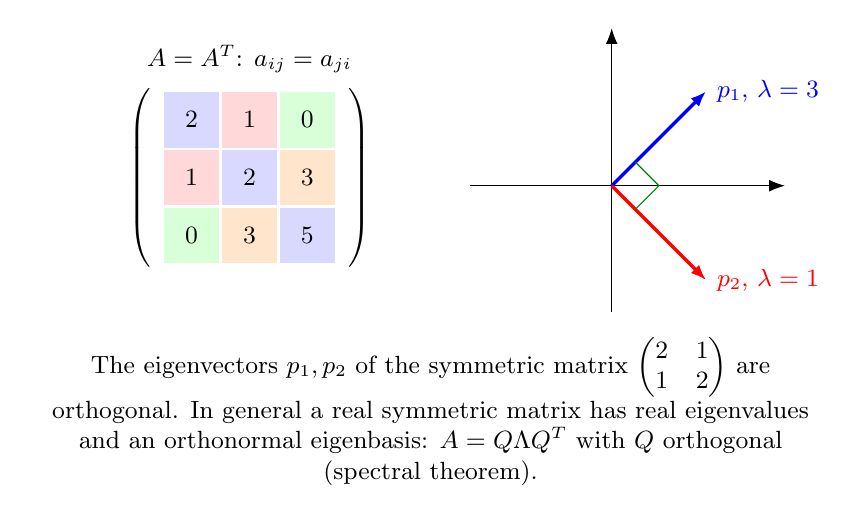
\begin{tikzpicture}[every node/.style={font=\small}, >={Latex[length=2mm]}]
	\matrix (A) [matrix of math nodes, nodes={minimum size=7mm, anchor=center}, left delimiter=(, right delimiter=), column sep=1pt, row sep=1pt] at (0,0) {
		|[fill=blue!15]| 2 & |[fill=red!15]| 1 & |[fill=green!15]| 0 \\
		|[fill=red!15]| 1 & |[fill=blue!15]| 2 & |[fill=orange!20]| 3 \\
		|[fill=green!15]| 0 & |[fill=orange!20]| 3 & |[fill=blue!15]| 5 \\
	};
	\node[anchor=south] at (A.north) {$A=A^{T}$: $a_{ij}=a_{ji}$};
	\begin{scope}[xshift=4.6cm, yshift=-0.1cm]
		\draw[->] (-1.8,0) -- (2.2,0);
		\draw[->] (0,-1.6) -- (0,2.0);
		\draw[->, blue, very thick] (0,0) -- (1.2,1.2) node[right, font=\small] {$p_1$, $\lambda=3$};
		\draw[->, red, very thick] (0,0) -- (1.2,-1.2) node[right, font=\small] {$p_2$, $\lambda=1$};
		\draw[green!50!black] (0.3,0.3) -- (0.6,0) -- (0.3,-0.3);
	\end{scope}
	\node[anchor=north, align=flush center, text width=10cm] at (2.3,-1.9) {The eigenvectors $p_1,p_2$ of the symmetric matrix $\begin{pmatrix}2&1\\1&2\end{pmatrix}$ are orthogonal. In general a real symmetric matrix has real eigenvalues and an orthonormal eigenbasis: $A=Q\Lambda Q^{T}$ with $Q$ orthogonal (spectral theorem).};
\end{tikzpicture}
\end{document}
